\documentclass[letterpaper,12pt]{report}

\usepackage{latexsym}
\usepackage[empty]{fullpage}
\usepackage[left = 2cm, right = 2cm, top = 1.5cm, bottom = 1.5cm, footskip = 15pt]{geometry}
\usepackage{titlesec}
\titlelabel{\thetitle.\quad}
\usepackage{marvosym}
\usepackage[usenames,dvipsnames]{color}
\usepackage{verbatim}
\usepackage{enumitem}
\usepackage[hidelinks]{hyperref}
\hypersetup{
    colorlinks=true,      
    urlcolor=blue,
}
\usepackage{fancyhdr}
\usepackage{calc}
\usepackage[english]{babel}
\usepackage{tabularx}
\usepackage{kpfonts}
\usepackage[T1]{fontenc}
\usepackage{subcaption}
\usepackage{float}
\input{glyphtounicode}
\usepackage{graphicx} 
\graphicspath{{.}}

\tolerance=1
\emergencystretch=\maxdimen
\hyphenpenalty=10000
\hbadness=10000

\pagestyle{fancy}
% Clear the header and footer
\fancyhead{}
\fancyfoot{}
\renewcommand{\headrulewidth}{0pt}
% Set the right side of the footer to be the page number
\fancyfoot[C]{\thepage}


\begin{document}

{\centering
    \textbf{\Huge{Stochastic Processes Report}} \\ \vspace{5pt}
    \Large{Modelling and predicting Covid19 infections using the SIR model and MCMC sampling} \\
}
\begin{flushright}
\small{By Group 2: Sourodeep Datta, 21CS10064\\
Tanishq Prasad, 21CS30054\\
Anit Mangal, 21CS10005\\
Anwesha Das, 21CS30007\\
Mihir Mallick, 21CS30031\\
Soumik Mandal, 21CS10063}\\
Link to Repository: \href{https://github.com/TheLapisGoat/SIR-Model-with-MCMC-Analysis}{GitHub}
\end{flushright}

\section*{\large Data Scraping: } \vspace{-10pt}
The data was scraped from \href{https://www.worldometers.info/coronavirus/country/india/}{\color{Blue} WorldoMeters}, which keeps a copy of the data published by the Ministry of Health and Family Welfare. The data is a time series, starting from Feb 15, 2020, to March 22, 2023. The data consists of the Total Daily Cases, New Cases, Active Cases, Total Deaths, Daily Deaths, and New Recoveries. From there, the data used is the Active Cases (which is I), and the cumulative sum of the New Recoveries (which is R).
\vspace{-10pt}
\section*{\large The SIR Model:} \vspace{-10pt}
The SIR model is a compartmental model consisting of:\vspace{-5pt}
\begin{itemize}
    \item {S: The number of susceptible individuals. When a susceptible and an infectious individual come into "infectious contact", the susceptible individual contracts the disease and transitions to the infectious compartment.
    }\vspace{-5pt}
    \item {I: The number of infectious individuals. These are individuals who have been infected and are capable of infecting susceptible individuals.
    }\vspace{-5pt}
    \item {R: The number of removed (and immune) or deceased individuals. These are individuals who have been infected and have either recovered from the disease and entered the removed compartment or died. It is assumed that the number of deaths is negligible with respect to the total population.
    }
\end{itemize}\vspace{-5pt}

\noindent
The SIR system without vital dynamics (birth and death) can be described above can be expressed by the following system of ordinary differential equations: \\
\begin{equation}
    \scalebox{1.4}{$\frac{\mathrm{dS} }{\mathrm{d} t} = -\frac{\beta IS}{N}$}
\end{equation}
\begin{equation}
    \scalebox{1.4}{$\frac{\mathrm{dI} }{\mathrm{d} t} = \frac{\beta IS}{N} - \gamma I$}
\end{equation}
\begin{equation}
    \scalebox{1.4}{$\frac{\mathrm{dR} }{\mathrm{d} t} = \gamma I$}
\end{equation}
\begin{equation}
    \scalebox{1.2}{$S(t) + I(t) + R(t) = N$}
\end{equation}
\begin{equation}
    \scalebox{1.4}{$R_0 = \frac{\beta }{\gamma }$}
\end{equation}


\noindent
Here, $R_0$ is the basic reproduction number, the expected number of total cases generated by one active case. In our model, the N = 1366417754, which was the population of India in 2019. We aim to determine the values of $\beta$ and $\gamma$, given the data and some initial states, using a Metropolis Hastings sampler.\\ \vspace{-10pt}

\noindent
As the value of N and S tends to be high, when considering the data for India, in order to prevent numerical instability, we made the following change: \vspace{-5pt}
\begin{equation*}
    \scalebox{1.4}{$s = \frac{S}{N}$}    
\end{equation*} \vspace{-5pt}
This changes equations $(1)$ and $(2)$ to: \vspace{-5pt}
\begin{equation}
    \scalebox{1.4}{$\frac{\mathrm{ds} }{\mathrm{d} t} = -\frac{\beta Is}{N}$}
\end{equation}
\begin{equation}
    \scalebox{1.4}{$\frac{\mathrm{dI} }{\mathrm{d} t} = \beta Is - \gamma I$}
\end{equation} \vspace{-20pt}


\section*{\large Metropolis Hastings Algorithm:} \vspace{-10pt}
The Metropolis Hastings algorithm is a Markov chain Monte Carlo (MCMC) method for obtaining a sequence of random samples from a probability distribution from which direct sampling is difficult. This sequence can be used to approximate the distribution, in this case, being used to find the posterior distributions of $\beta$ and $\gamma$. \\ \vspace{-5pt}

\noindent
The algorithm for a symmetric proposal distribution (in our case a Normal Distribution) is: \vspace{-5pt}
\begin{enumerate}
    \item Choose an initial starting point $x_0$ form prior distributions and a proposal distribution $g(x | y)$. The proposal distribution suggests the next candidate $x$ given the previous sample value $y$. As $g(x | y)$ is assumed to be symmetrical, we can say $g(x | y) = g(y | x)$. \vspace{-5pt}
    \item For each iteration t: \vspace{-5pt}
    \begin{enumerate}
        \item Sample a candidate $x'$ from $g(x|y)$. \vspace{-2pt}
        \item Calculate the acceptance ration $\alpha = \frac{f(x')}{f(x_t)}$. \vspace{-2pt}
        \item Accept or reject the candidate by sampling $u$ from a $U(0, 1)$ distribution. If $u \leq \alpha$, accept it, otherwise reject it.  
    \end{enumerate}
\end{enumerate} \vspace{-5pt}

\noindent
In our model, we use the DEMetropolisZ Algorithm, which is an extension of the Metropolis Hastings Algorithm.
\vspace{-10pt}

\section*{\large Calculating $\beta$ and $\gamma$:}\vspace{-10pt}
The data collected is for a large period of time, and the three major covid waves are visible in it. The SIR model is meant for only a single wave, so we clip the first and second waves and only consider data gathered from day number 800 (Considering the start day to be 0).


\begin{figure}[H]
\begin{subfigure}{0.5\textwidth}
\hspace{-25pt}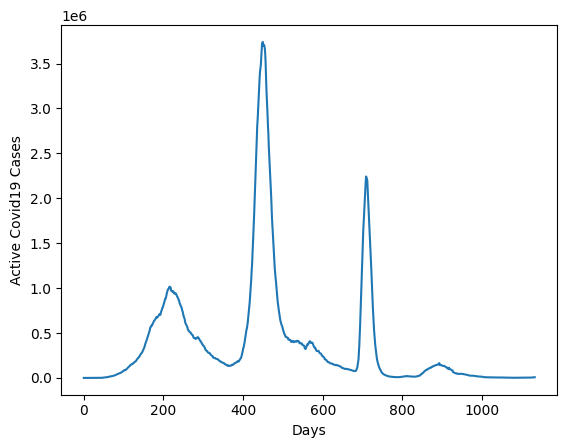
\includegraphics[scale=0.62]{I.png}
\caption{Active Cases v/s Days for all waves}
\end{subfigure}
\begin{subfigure}{0.5\textwidth}
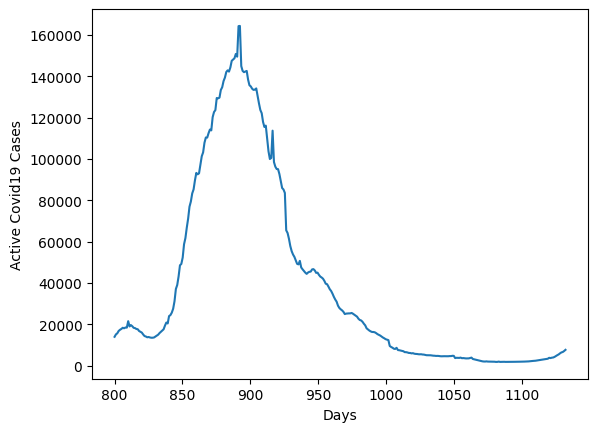
\includegraphics[scale=0.62]{I_new.png}
\caption{Active Cases v/s Days from day 800}
\end{subfigure}
\end{figure}

\noindent
Similarly, the data for S and R is also truncated. This is then used to make a hierarchical bayesian model, with the number of active cases being assumed to be a Poisson process, with means being dependent on the ODE, which in turn is dependent on beta and gamma, which are sampled from LogNormal prior distributions, with hyperparameters being based on empirical data.
\begin{equation*}
    \scalebox{1.2}{$\beta \sim LogNormal\left (log(0.4), 0.5 \right )$}
\end{equation*}
\begin{equation*}
    \scalebox{1.2}{$\gamma \sim LogNormal\left (log(0.125), 0.2 \right )$}
\end{equation*}

\begin{figure}[H]
    \centering
    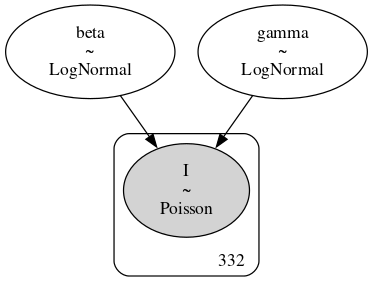
\includegraphics[scale = 0.51]{model.png}
    \caption{Bayesian Model}
    \label{fig:my_label}
\end{figure}

\noindent
After creating the model, we ran the sampler for $4$ chains, each with $21000$ samples, out of which $1000$ are for tuning. This leads to a total of $84000$ samples. The trace plots for the samples are:

\begin{figure}[H]
    \centering
    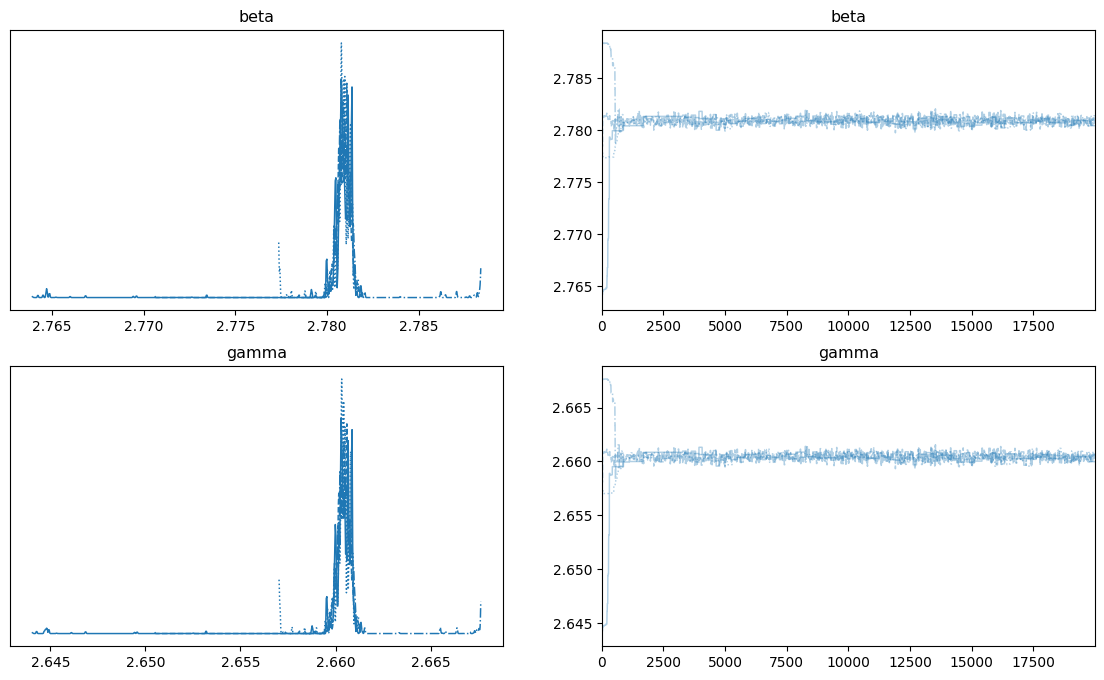
\includegraphics[scale = 0.65]{trace.png}
    \caption{Trace}
\end{figure}

\noindent
We take the first 1000 iterations to be burn-in, and so slice them off. The remaining trace is the burned trace.

\begin{figure}[H]
    \centering
    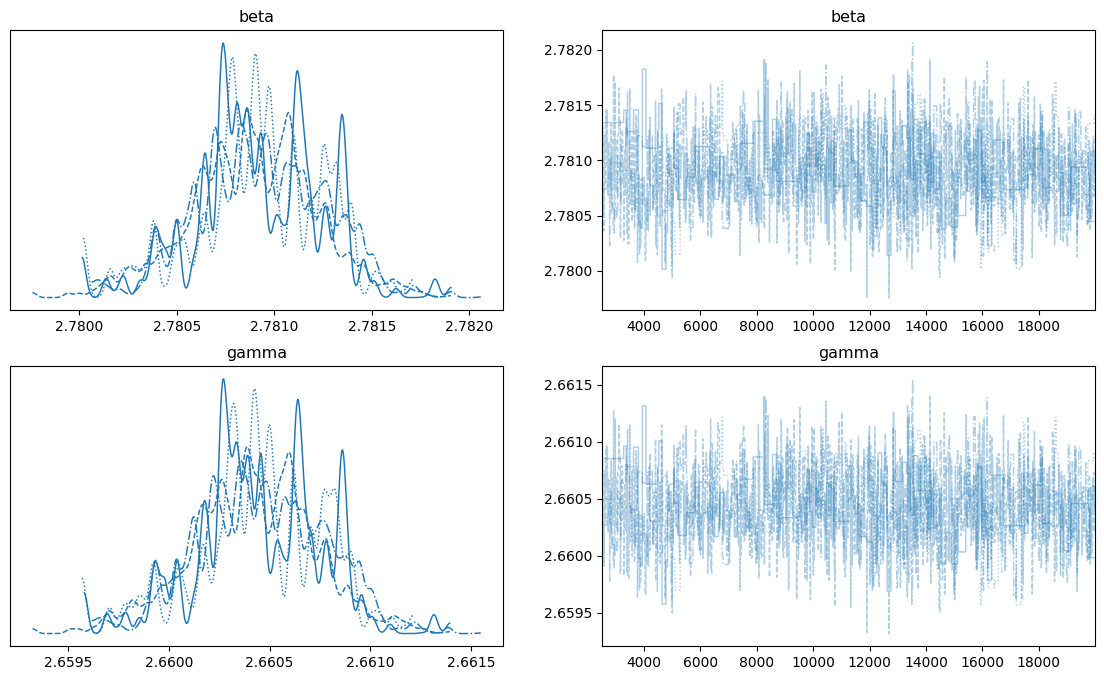
\includegraphics[scale = 0.59]{trace_burned.png}
    \caption{Burned Trace}
\end{figure}

\noindent
The posterior distributions of $\beta$ and $\gamma$ have been found. Using them, we can find their means to be 2.781 and 2.660 respectively.

\begin{figure}[H]
    \centering
    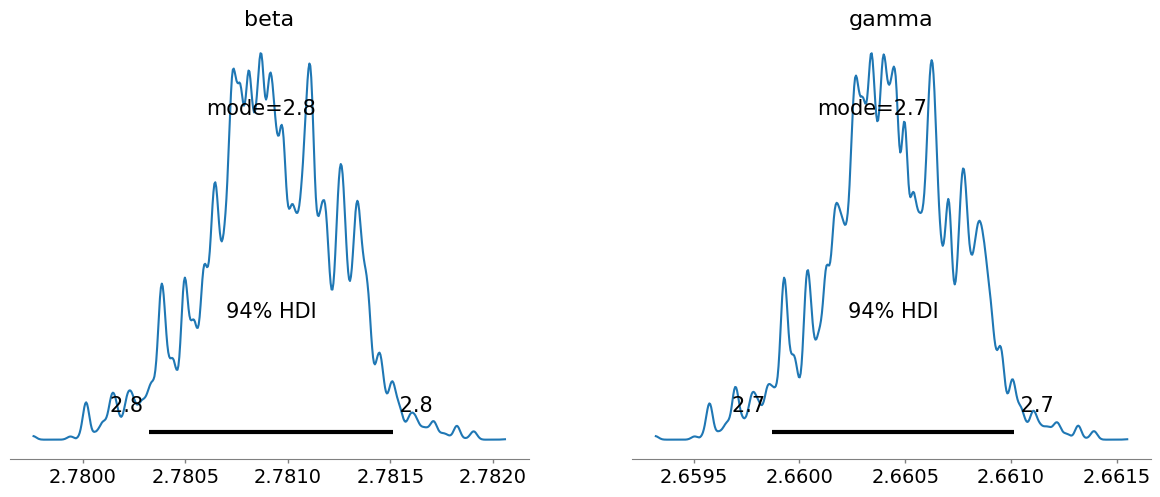
\includegraphics[scale = 0.61]{burned_posterior.png}
    \caption{Posterior of $\beta$ and $\gamma$}
\end{figure}

\noindent
Using these values, we can calculate $R_0$, which is 1.045. Using this, we predict the number of active cases on March 23, 2023 (our data used to make the model was till March 22, 2023) to be 7950. Based on the actual data, it is found to be 7927. Thus, our estimate is very close to the actual data.\\

\begin{figure}[H]
\centering
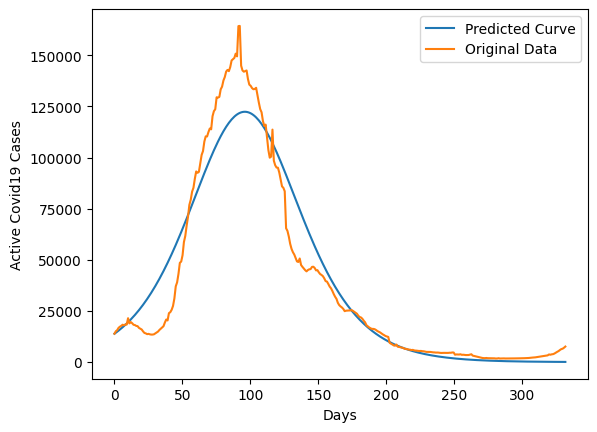
\includegraphics[scale=0.9]{Prediction+Data.png}
\caption{Predicted Active Cases Curve}
\end{figure}

\section*{\large Conclusion:}
The SIR model is one of the simplest compartmental models, and is reasonably effective for making predictions on diseases where recovery confers lifelong immunity. Covid19 is not one such disease, as reinfection is possible, and so we can not expect it to be able to model the disease well. Nevertheless, this model serves as the base for many other compartmental models, such as the SEIS and SIRV models, which are better suited for modelling Covid19. This project is an exercise on the application of various mathematical tools and methods which can be used for the epidemiological modelling of infectious diseases. By applying mathematical methods and tools to real-world data, we can gain valuable insights into how diseases like Covid19 are spreading, and what measures might be most effective in slowing or preventing their spread. Overall, this project has highlighted the importance of mathematical modelling in epidemiology, and the potential it holds for helping us better understand and combat infectious diseases.

\end{document}